\documentclass{standalone}

\usepackage{tikz}

\definecolor{myBlue}{RGB}{56, 77, 193}

\begin{document}
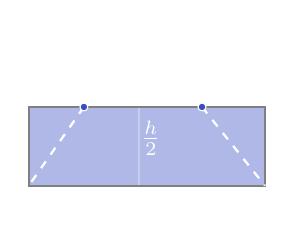
\begin{tikzpicture}
  \draw [thick,fill=myBlue, opacity=0.4] (0,0) rectangle (3,1);
  \node[white] at (2,-0.2) {$ b $};
  \draw[thick,white,opacity=0.3] (1.4,1)--(1.4,0);
  \node[white] at (1.55,0.6) {$ \frac{h}{2} $};
  \draw[green,opacity=0] (0.5,1.9) circle (0.1);
  \draw[color=gray,thick,opacity=1] (0,0)--(3,0)--(3,1)--(0,1)--(0,0)--(3,0);
  \draw[white, thick, dashed] (0.7,1)--(0,0);
  \draw[white, thick, dashed] (2.2,1)--(3,0);
  \draw[white, fill=myBlue] (0.7,1) circle (0.05);
  \draw[white, fill=myBlue] (2.2,1) circle (0.05);
\end{tikzpicture}	
\end{document}